\doublespacing % Do not change - required

\chapter{Method and Implementation}
\label{ch:method-implementation}

%%%%%%%%%%%%%%%%%%%%%%%%%%%%%%%%%%%%%%%
% IMPORTANT
\begin{spacing}{1}
\minitoc
\end{spacing}
\thesisspacing
%%%%%%%%%%%%%%%%%%%%%%%%%%%%%%%%%%%%%%%

\begin{bodytwocol}

\section{Overview}

This chapter describes the implemented aggregation method, \textbf{HRAC}
(History-Residual Adaptive Clipping). HRAC is a server-side defence for
federated learning under Byzantine behaviour. It is implemented in PyTorch in
the \texttt{C\_HRAC} aggregation class and is integrated into the centralised
training pipeline through the common \texttt{CentraliedAggregation} interface.

The design goal is to reduce malicious influence without forcing all benign
clients into one tight cluster. This is important under non-IID data: a benign
client may consistently differ from the population mean because its local data
distribution is different. HRAC therefore uses each client's own history as the
main reference. The method combines (i) a robust global norm cap, (ii)
per-client history-residual clipping, (iii) residual-change tracking through
EMA statistics, and (iv) a late-stage soft weighting rule based on elevated
change statistics.

\section{Aggregation Pipeline}

In communication round $t$, the server receives flattened client updates
$\{\Delta_i^t\}_{i=1}^{N}$, with $\Delta_i^t \in \mathbb{R}^d$. The pipeline is:

\begin{enumerate}[leftmargin=*, itemsep=0.2em, topsep=0.2em]
    \item \textbf{State initialisation.}
    For a new client, initialise its historical centre $b_i$, residual scale
    $\mu_i$, change statistic $\nu_i$, and previous clipped residual.

    \item \textbf{Global robust clipping.}
    Clip every update to a round-wise cap proportional to the median update norm.

    \item \textbf{History-residual clipping.}
    Compare each clipped update with that client's own EMA history centre, then
    clip only the residual.

    \item \textbf{Residual-change tracking.}
    Update $\mu_i$ and $\nu_i$ using EMA recursions computed from the clipped
    residual path.

    \item \textbf{Soft weighting and aggregation.}
    Before the $\nu$ penalty is activated, use uniform weights. Afterwards,
    reduce the weights of clients whose $\nu_i$ values exceed the population
    baseline and the activation threshold.

    \item \textbf{History update and logging.}
    Update per-client histories and record diagnostic values for later analysis.
\end{enumerate}

\section{Core Components}

\subsection{Global Median Norm Cap}

The first defence layer prevents a single large update from dominating the
aggregate. Let
\[
    m_t = \operatorname{med}_{1\leq j\leq N}\|\Delta_j^t\|_2,
    \qquad
    B_t = c_g m_t ,
\]
where $c_g$ is a fixed multiplier. Each update is clipped by
\begin{equation}
    \hat{\Delta}_i^t
    =
    \min\!\left(1,\frac{B_t}{\|\Delta_i^t\|_2+\epsilon}\right)\Delta_i^t .
\end{equation}
The implementation uses $c_g=3.0$ by default. This cap is deliberately
round-wise and median-based: it does not require knowing which clients are
malicious, and it is less sensitive to extreme Byzantine norms than a mean-based
scale estimate.

\subsection{Per-Client History-Residual Clipping}

For each client $i$, HRAC stores a historical centre $b_i^t$. This centre is an
EMA of safe past messages and represents the client's own typical update path,
not a population-wide prototype. The residual is
\begin{equation}
    r_i^t = \hat{\Delta}_i^t - b_i^t .
\end{equation}
The residual threshold is adaptive:
\begin{equation}
    \tau_i^t = c\mu_i^t + \epsilon ,
\end{equation}
where $\mu_i^t$ is an EMA scale statistic and $c=2.5$ by default. The clipped
residual is
\begin{equation}
    \bar r_i^t
    =
    \min\!\left(1,\frac{\tau_i^t}{\|r_i^t\|_2+\epsilon}\right)r_i^t .
\end{equation}
The processed message is then reconstructed as
\begin{equation}
    \tilde{\Delta}_i^t = b_i^t + \bar r_i^t .
\end{equation}
An optional post-residual cap re-applies the global cap to
$\tilde{\Delta}_i^t$. This option is enabled in the current implementation and
prevents the reconstruction step from reintroducing a message whose norm
exceeds $B_t$.

\subsection{Separated Aggregation and Statistics Paths}

The implementation distinguishes the aggregation path from the statistics path.
Aggregation uses the globally clipped update $\hat{\Delta}_i^t$ and its
processed version $\tilde{\Delta}_i^t$. The statistics path can lift extremely
small-norm updates to the median norm when computing $\mu_i$ and $\nu_i$. This
prevents a near-zero update from artificially collapsing a client's history
statistics. The aggregation value itself is not lifted in this case, so the
actual model update remains faithful to the received message after global
clipping.

\subsection{EMA History Updates}

After aggregation, HRAC updates the client histories. The aggregation-path
centre is
\begin{equation}
    b_i^{t+1}
    =
    \rho_b b_i^t + (1-\rho_b)\Delta_{i,\mathrm{safe}}^t ,
\end{equation}
where $\Delta_{i,\mathrm{safe}}^t$ is the processed message after the safety cap.
The default value is $\rho_b=0.98$.

The residual scale statistic is updated as
\begin{equation}
    \mu_i^{t+1}
    =
    \rho_\mu \mu_i^t + (1-\rho_\mu)\|\bar r_i^t\|_2 ,
\end{equation}
with a small floor $\mu_{\min}$ for numerical stability. The default is
$\rho_\mu=0.95$.

The change statistic $\nu_i$ is updated from the movement of the clipped
residual:
\begin{equation}
    d_i^t = \|\bar r_i^t - \bar r_i^{t-1}\|_2 ,
    \qquad
    \nu_i^{t+1}
    =
    \rho_\nu \nu_i^t + (1-\rho_\nu)d_i^t ,
\end{equation}
again with a small floor $\nu_{\min}$. The default is $\rho_\nu=0.95$.

\subsection{Soft Weighting from the $\nu$ Statistic}

HRAC does not immediately down-weight clients from the first round. For
iterations $t \leq T_{\nu}$, it uses uniform weights. In the implementation,
$T_{\nu}=50$ by default. This warm-up allows the per-client statistics to become
meaningful before they affect aggregation.

Once the penalty is active, the server forms a population baseline
\begin{equation}
    \bar{\nu}^t = \frac{1}{N}\sum_{j=1}^{N}\nu_j^t .
\end{equation}
Only clients with sufficiently high $\nu_i^t$ are penalised. In code, the
activation threshold is $0.9$, and the excess score is
\begin{equation}
    e_i^t =
    \begin{cases}
        \max(\nu_i^t-\bar{\nu}^t,0), & \nu_i^t>0.9,\\
        0, & \nu_i^t\leq 0.9 .
    \end{cases}
\end{equation}
The raw weight is
\begin{equation}
    \hat w_i^t = \frac{1}{1+\alpha e_i^t},
\end{equation}
where $\alpha=5.0$ by default. Raw weights are normalised to sum to one. A
maximum per-client weight cap, $w_{\max}=0.30$, is then applied iteratively with
renormalisation to avoid a small number of clients dominating the round.

The final aggregate is
\begin{equation}
    g_t = \sum_{i=1}^{N} w_i^t\tilde{\Delta}_i^t .
\end{equation}

\section{Hyperparameters}

The main HRAC hyperparameters are:
\begin{itemize}[leftmargin=*]
    \item $\rho_b=0.98$: EMA decay for the client history centre.
    \item $\rho_\mu=0.95$: EMA decay for the residual scale statistic.
    \item $\rho_\nu=0.95$: EMA decay for the residual-change statistic.
    \item $c=2.5$: multiplier for the per-client residual clipping threshold.
    \item $c_g=3.0$: multiplier for the global median norm cap.
    \item $T_\nu=50$: first iteration after which $\nu$-based weighting is used.
    \item $\alpha=5.0$: strength of the $\nu$ excess penalty.
    \item $w_{\max}=0.30$: maximum normalised weight allowed for one client.
\end{itemize}

The algorithm is intentionally not a hard detector. Client identities are used
only for controlled logging and evaluation; the aggregation rule itself does not
need attacker labels or the attacker fraction.

\section{Preliminary Results}
\label{sec:prelim-results}

This section reports \emph{sanity-check} experiments that validate our end-to-end FL evaluation pipeline
(data partitioning, attack injection, logging, and aggregation hooks) and reproduce representative baseline
phenomena reported in prior work. These results are \emph{not} claimed as the final evaluation of
HRAC; rather, they serve two purposes: (i) demonstrating that the experimental framework is
functioning correctly, and (ii) motivating the design choices of HRAC (global robust clipping,
per-client residual histories, and soft $\nu$-based weighting) under heterogeneous regimes.
Where applicable, the experimental protocol is aligned with the setup in \cite{ijcai2024p530}.

Unless otherwise stated, we use CIFAR-10 with Byzantine contamination level $b=3$ (i.e., $30\%$ malicious
clients among the participating clients per round). In addition to test accuracy, the implementation logs
diagnostic quantities including residual thresholds $\tau_i$, scale statistics $\mu_i$,
change statistics $\nu_i$, normalised aggregation weights, and attacker-aware bottom-weight summaries in
controlled settings.

\paragraph{MSA / shuffle-style attack.}
Figure~\ref{fig:prelim-msa} illustrates a structural manipulation setting where attackers disrupt coordinate
structure (e.g., shuffling-style behaviors). Methods that rely strongly on coordinate geometry can exhibit
instability, as the apparent direction and internal structure of updates become inconsistent across clients.
HRAC is designed to mitigate this failure mode by first limiting update norms with a median-based cap, then
comparing each client against its own residual history. This avoids relying on a single global cluster while
still reducing the effect of abrupt or high-magnitude manipulated updates.

\paragraph{History-aware attack (HisMSA).}
Figure~\ref{fig:prelim-hismsa} stresses temporal vulnerability: small but persistent perturbations can
accumulate through server-side history and induce long-term bias. In such settings, within-round checks may
appear stable early on yet degrade later as bias compounds. HRAC explicitly tracks per-client residual
behaviour across rounds. Persistent residual movement raises the $\nu_i$ statistic; after the warm-up period,
clients with elevated $\nu_i$ relative to the population are softly down-weighted.

\paragraph{Label-flipping poisoning.}
Figure~\ref{fig:prelim-lf} corresponds to a practical poisoning scenario where corrupted local objectives
produce plausible-looking updates. A key observation in the literature is that under certain non-IID
conditions, simple averaging (\textsc{Mean}) can remain surprisingly competitive relative to some robust
rules that over-suppress benign heterogeneous clients \cite{ijcai2024p530}. We include this setting mainly
as a pipeline validation and a baseline reference point. It also motivates our \emph{soft} and
\emph{relative} weighting design: HRAC avoids comparing every client to a single population centre and uses
client-specific histories to reduce the risk of ``false positives'' on benign non-IID updates while still
attenuating coordinated malicious influence.

\medskip
These results are preliminary and primarily motivate the full evaluation in the final dissertation.
The final study will extend the comparison to additional datasets and stronger baseline aggregators
(e.g., Trimmed Mean, Median, Krum, RFA, FLTrust) under matched training budgets, together with ablations
that isolate the contribution of each component of HRAC. Additional plots (more seeds/partitions)
will be provided in the Appendix.

\end{bodytwocol}

\begin{figure}[t]
    \centering
    \begin{subfigure}[t]{0.32\textwidth}
        \centering
        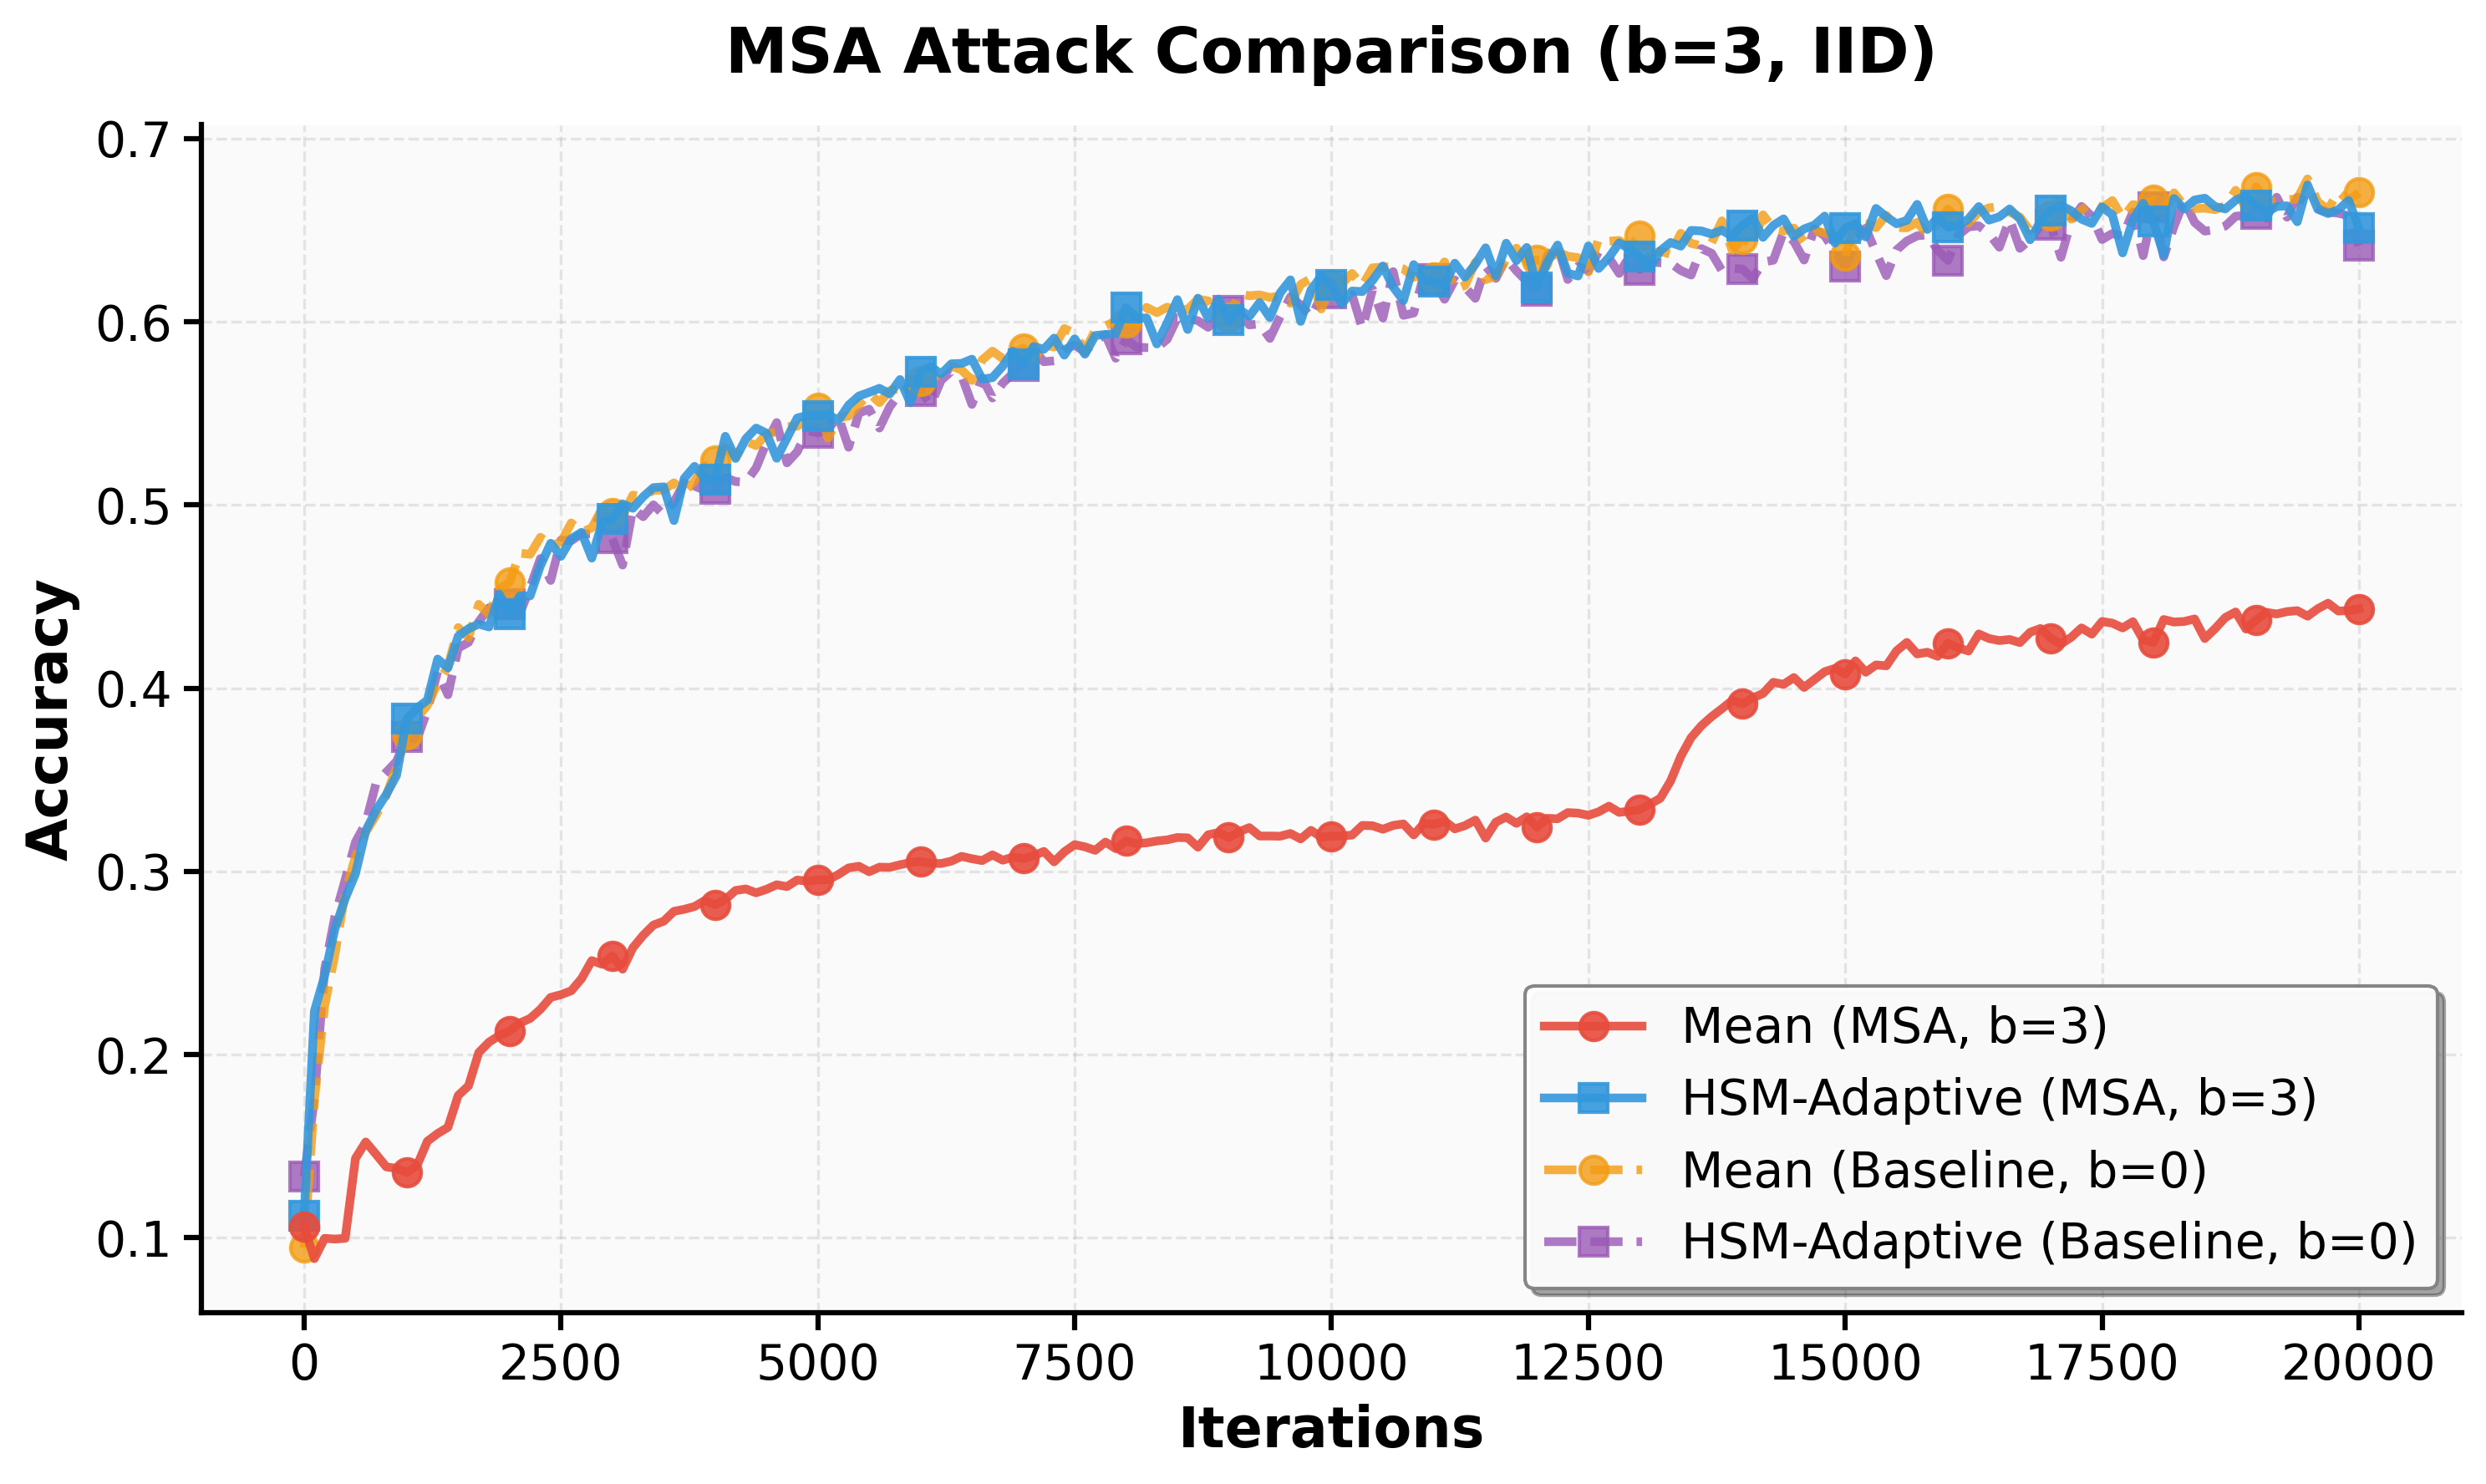
\includegraphics[width=\linewidth]{imgs/CMomentum_cifar10_MSA_b3_comparison}
        \caption{CIFAR-10 under MSA/shuffle-style attack.}
        \label{fig:prelim-msa}
    \end{subfigure}\hfill
    \begin{subfigure}[t]{0.32\textwidth}
        \centering
        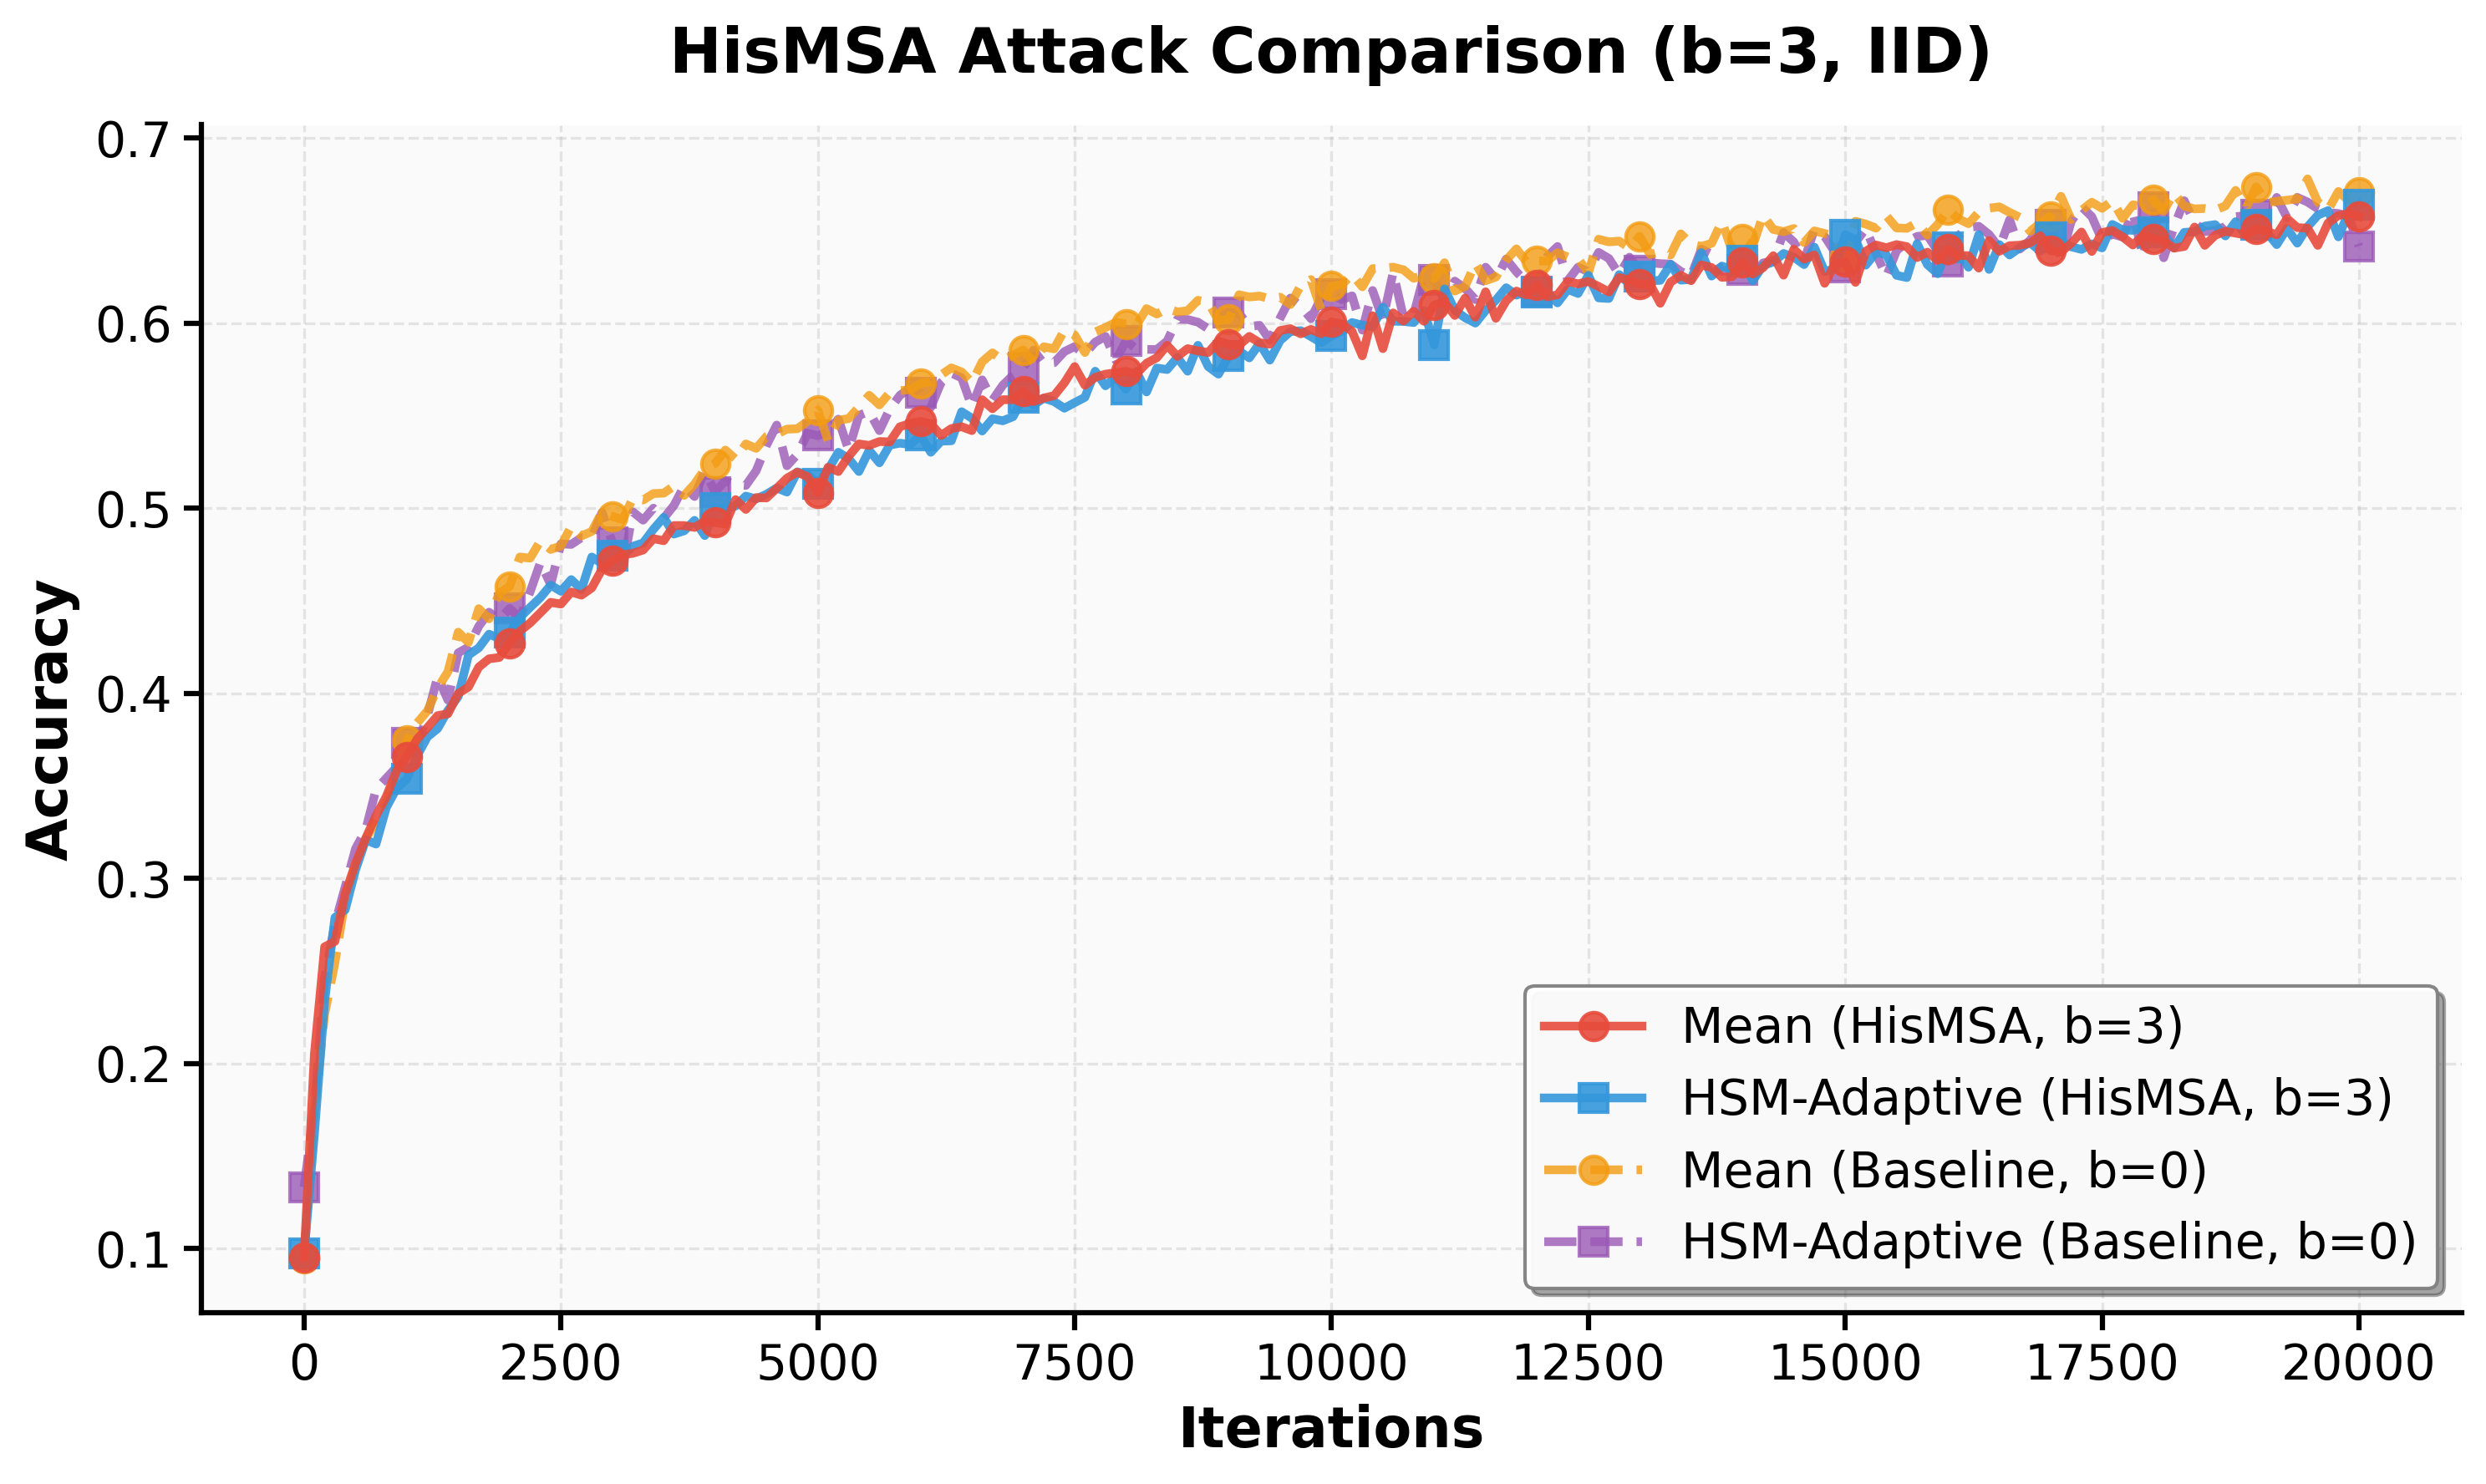
\includegraphics[width=\linewidth]{imgs/CMomentum_cifar10_HisMSA_b3_comparison}
        \caption{CIFAR-10 under history-aware (HisMSA) attack.}
        \label{fig:prelim-hismsa}
    \end{subfigure}\hfill
    \begin{subfigure}[t]{0.32\textwidth}
        \centering
        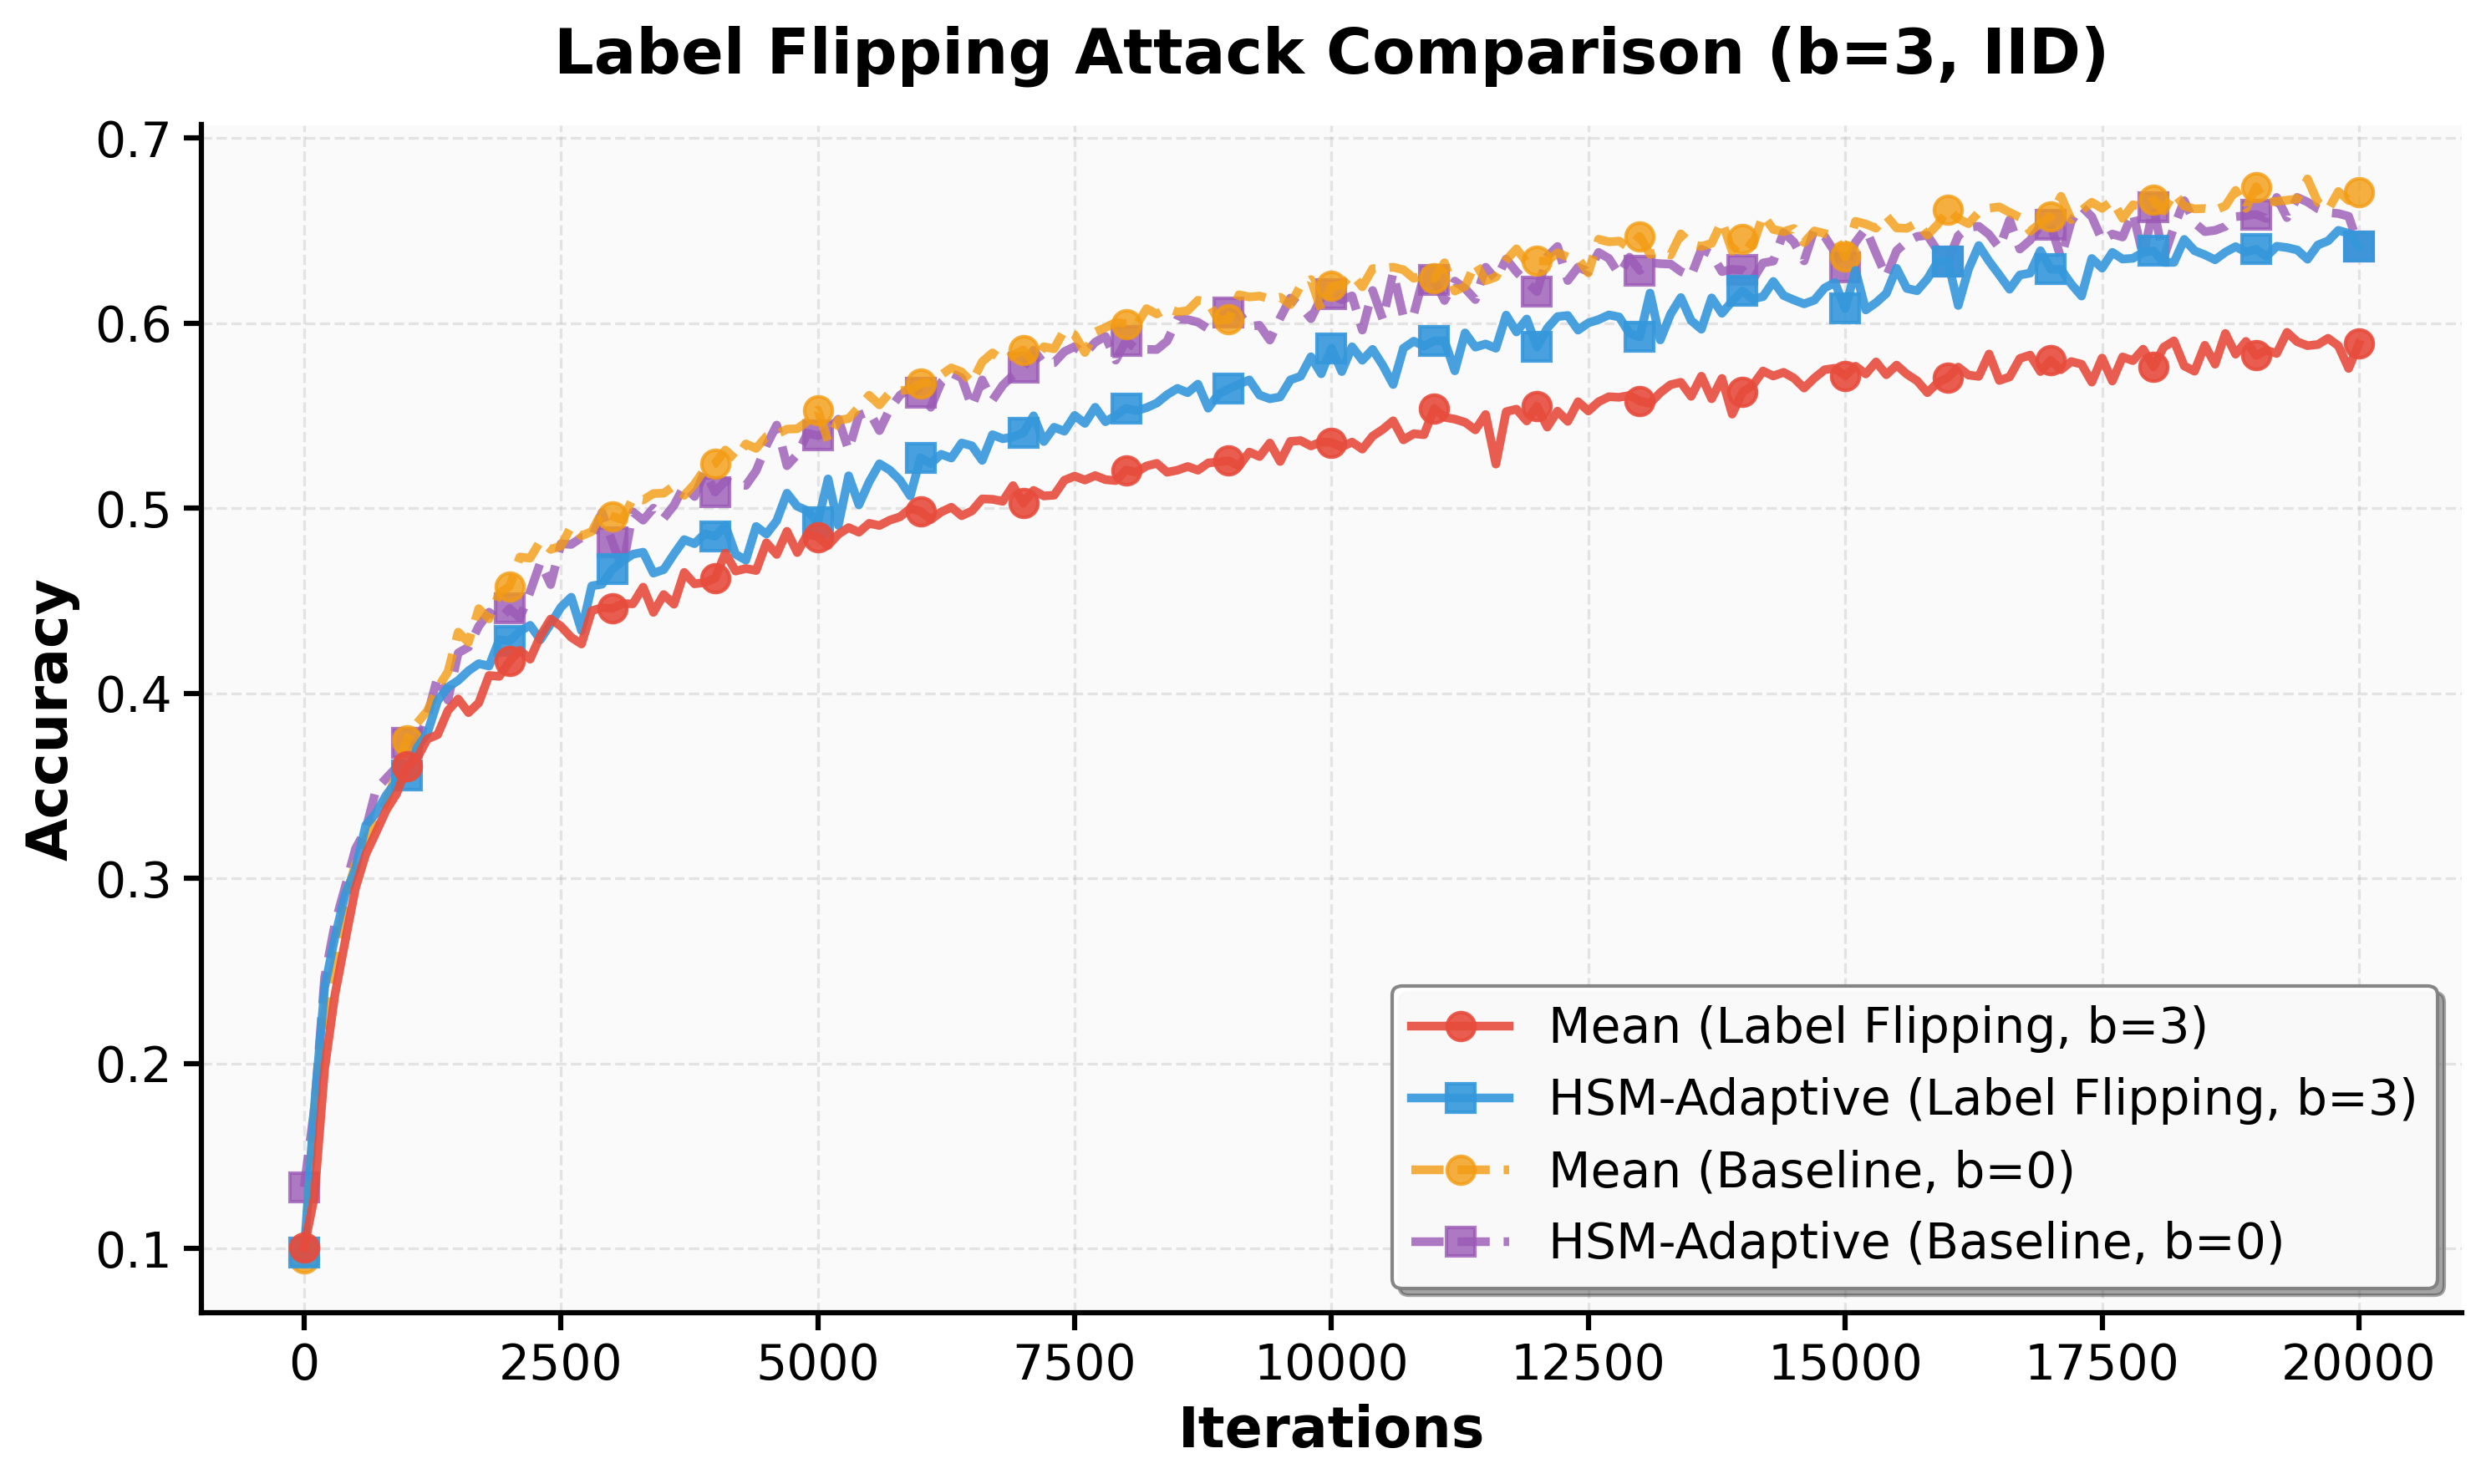
\includegraphics[width=\linewidth]{imgs/CMomentum_cifar10_label_flipping_b3_comparison}
        \caption{CIFAR-10 under label-flipping poisoning (\textsc{Mean} baseline reproduction).}
        \label{fig:prelim-lf}
    \end{subfigure}
    \caption{Preliminary robustness comparison on CIFAR-10 across three threat settings ($b=3$).
    Curves show test accuracy over communication rounds for different aggregators.
    Results are produced by our implementation; the label-flipping baseline setting follows the protocol
    in \cite{ijcai2024p530} (used here primarily as a sanity-check and reference baseline).}
    \label{fig:prelim-results}
\end{figure}
